\chapter{Sung keyword spotting} \label{chap:kws}
Keyword spotting is another task for which the new acoustic models described in chapter \ref{chap:phonerec} were employed. A keyword-filler HMM algorithm was selected due to its independence on phoneme durations, which is a condition that cannot be fulfilled easily in singing. As described in section \ref{sec:tech_kwfhmm}, keyword-filler HMMs consist of two sub-HMMs: One to model the keyword and one to model everything else (=filler). The keyword HMM has a simple left-to-right topology with one state per keyword phoneme. The filler HMM is a fully connected loop of all phonemes. When the Viterbi path with the highest likelihood passes through the keyword HMM rather than the filler loop, the keyword is detected. Keyword detection was performed on whole songs, which is a realistic assumption for many practical applications. The \textit{ACAP} and \textit{DampTest} data sets were used for evaluation with the keyword set described in section \ref{sec:data_kws}. Song-wise $F_1$ measures were calculated for evaluation.

\section{Keyword spotting using keyword-filler HMMs}
\subsection{Comparison of acoustic models}
Phoneme posteriorgrams were generated with the various acoustic models described in section \ref{sec:phonerec_acap}. The results in terms of $F_1$ measure across the whole \textit{DampTest} sets are shown in figure \ref{fig:kws_exp1}. Figure \ref{fig:kws_exp1_acap} show the results of the same experiment on the small \textit{ACAP} data set.

Across all keywords, a document-wise $F_1$ measure of $0.44$ is obtained using the posteriorgrams generated with the \textit{TIMIT} model on the \textit{DampTest} data sets. This result remains the same for the \textit{TimitM} models trained on ``songified'' speech. In this experiment, using models trained on the \textit{DAMP}-based singing data sets only improves the results slightly, with $F_1$ measures of $0.47$ for the \textit{DampB} model, and $0.46$ with the much smaller \textit{DampBB\_small} model. Surprisingly, in this case, the model trained on the medium-size balanced data set \textit{DampBB} performs a little worse than the smallest one; however, this might just be due to some statistical fluctuation. In general, results on these test data sets are somewhat inconclusive. There are several reasons for this: First, the annotations were generated automatically and the keywords were picked from the aligned lyrics. However, the singers may not always perform them or might pronounce them wrong. Additionally, the keyword approach can be tuned easily for high recall; then, the precision becomes the deciding factor for $F_1$ calculation. Considering the size of the data set, keyword occurrences are relatively rare, which makes obtaining a high precision more difficult and blurs the $F_1$ measures between approaches.\\

On the hand-annotated \textit{ACAP} test set, the differences are someqhat more pronounced. The $F_1$ measure is $0.48$ for the \textit{TIMIT} model, and rises to $0.52$ with the \textit{DampB} model. The \textit{TimitM} and \textit{DampBB}�models both produce $F_1$ measures of $0.49$. The higher over-all values could be caused by the more accurate annotations or by the higher-quality singing. Additionally, the data set is much smaller with fewer occurrences of each keyword, which could emphasize both positive and negative tendencies in the detection.\\

In general, recalls are usually close to $1$, and precisions often in the range of $0.2$ to $0.5$ (with much lower and higher outliers). For this reason, an approach that could exploit a configuration with high recalls and then discard unlikely occurrences could offer an improvement. This idea is explored further in section \ref{sec:kws_duration}.

\begin{figure}
        \centering
        \begin{subfigure}[t]{0.5\textwidth}
		 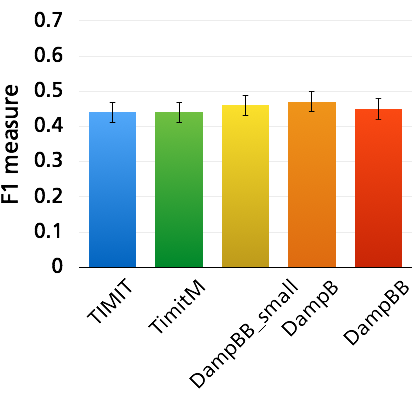
\includegraphics[width=\textwidth]{images/kws_exp1.png}
                \caption{\textit{DampTest}}
                \label{fig:kws_exp1}

        \end{subfigure}%
         %add desired spacing between images, e. g. ~, \quad, \qquad, \hfill etc.
          %(or a blank line to force the subfigure onto a new line)
        \begin{subfigure}[t]{0.5\textwidth}
                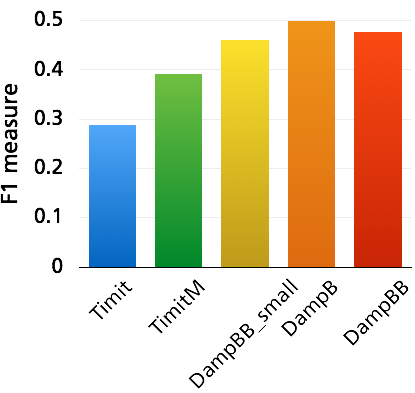
\includegraphics[width=\textwidth]{images/kws_exp1_acap.png}
                \caption{\textit{ACAP}}
                \label{fig:kws_exp1a}
        \end{subfigure}
        \caption{$F_1$ measures for keyword spotting results using posteriorgrams generated with various acoustic models.}
          \end{figure}
%\vspace{-5px}

\subsection{Gender-specific acoustic models}
%TODO: ACAP??
Keyword spotting was also performed on the posteriorgrams generated with the gender-dependent models trained on \textit{DampF} and \textit{DampM} (also described in section \ref{sec:phonerec_acap}. The results are shown in figure \ref{fig:kws_exp2}.

In contrast to the phoneme recognition results from Experiment C, the gender-dependent models perform slightly better for keyword spotting than the mixed one of the same size, and almost as good as the one trained on much more data (\textit{DampB}). The $F_1$ measures for the female test set are  $0.48$ for the \textit{DampB} model, $0.45$ for the \textit{DampBB} model, and $0.46$ for the \textit{DampFB} model. For the male test set, they are $0.46$ and $0.45$ for the first two, and $0.46$ for the \textit{DampMB} model.



\subsection{Individual analysis of keyword results}
%TODO: ACAP??
Figure \ref{fig:kws_exp3} shows the individual $F_1$ measures for each keyword using the best model (\textit{DampB}), ordered by their occurrence in the \textit{DampTest} sets from high to low (i.e. number of songs which include the song). There appears to be a tendency for more frequent keywords to be detected more accurately. This happens because a high recall is often achievable, while the precision depends very much on the accuracy of the input posteriorgrams. The more frequent a keyword, the easier it also becomes to achieve a higher precision for it.

As shown in literature \cite{phdthesis:thambiratnam}, the detection accuracy also depends on the length of the keyword: Keywords with more phonemes are usually easier to detect. This might explain the relative peak for ``every", in contrast to ``eyes" or ``world". Since keyword detection systems tend to perform better for longer words and most of the keywords only have 3 or 4 phonemes, this result is especially interesting.

One potential source of error are sequences of phonemes that overlap with keywords, but are not included in the calculation of the precision. Words spelled the same were included, but split phrases or other spellings were not (e.g. ``away" as part of ``castaway" would be counted, but ``a way" would not be counted as ``away"). This might artificially lower the results and could be an avenue for future improvement. Additionally, only one pronunciation for each keyword was provided, but there may be several possible.

\begin{figure}
 \begin{center}
                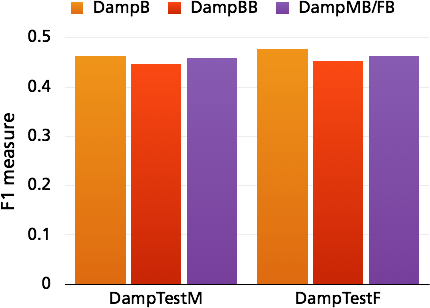
\includegraphics[width=0.5\textwidth]{images/kws_exp2.png}
                \caption{$F_1$ measures for keyword spotting results on the \textit{DampTestM} and \textit{DampTestF} data sets using mixed and gender-dependent models.}
                \label{fig:kws_exp2}
                 \end{center}
 \end{figure}

\begin{figure}
 \begin{center}
% 	\begin{subfigure}[t]{0.4\textwidth}
                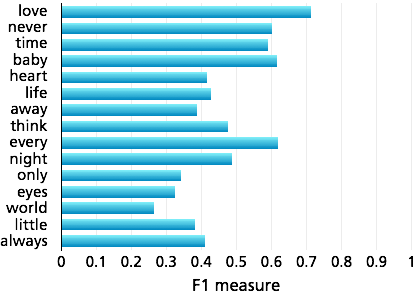
\includegraphics[width=.5\textwidth]{images/kws_exp3.png}
%               \caption{\textit{DampTest}}
%                \label{fig:kws_exp3_damp}
%       	\end{subfigure}
% 	\begin{subfigure}[t]{0.4\textwidth}
% 		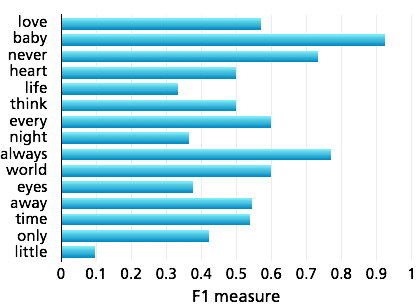
\includegraphics[width=\textwidth]{images/kws_exp3_acap.png}
% 		\caption{\textit{ACAP}}
% 		\label{fig:kws_exp3_acap}
% 	\end{subfigure}
       	
     	 \caption{Individual $F_1$ measures for the results for each keyword, using the acoustic model trained on \textit{DampB}.} 		\label{fig:kws_exp3}
                 \end{center}
 \end{figure}
%\vspace{-5px}





\section{Keyword spotting using duration-informed keyword-filler HMMs}\label{sec:kws_duration}
\subsection{Approach}
As mentioned above, a high recall is easily achievable with the described approach, but the comparatively low precision decreases the over-all result. Therefore, using additional information to sort out false positives would be a helpful next step.\\
One such source of information are the durations of the detected phonemes. As shown in figure \ref{fig:phone_durations}, each phoneme in the \textit{TIMIT} speech database has a fairly fixed duration. In singing, the vowels' durations vary a lot, but the consonants' are still quite predictable. Standard HMMs do not impose any restrictions on the state durations, resulting in a geometric distribution which does not correspond to naturally observed phoneme durations.\\
As first described in \cite{ferguson}, introducing restrictions on state durations can improve the recognition results. In \cite{juang}, Juang et al. present two basic approaches for duration modeling in HMMs: Internal duration modeling and Post-processor duration modeling.\\

In both approaches, parametric state duration models for each phoneme need to be calculated first \cite{levinson}. Several distributions has been tested for this task (e.g. Gaussian), but Burshtein showed that Gamma distributions are best at modeling naturally occurring phoneme duration distributions \cite{burshtein}:
\begin{equation}\label{eq:d}
d(\tau) = K \exp \{ - \alpha \tau \} \tau^{p-1}
\end{equation}
where $\tau = 0,1,2,...$ are the possible state durations in frames and $K$ is a normalizing factor. The parameters $\alpha$ and $p$ are estimated according to
\begin{equation}
\hat{\alpha} = \frac{E \{\tau\}}{VAR\{\tau\}} , \hat{p} = \frac{E^{2} \{\tau\}}{VAR\{\tau\}}
\end{equation}
where $E$ is the distribution mean and $VAR$ is the distribution variance. $E$ and $VAR$ are estimated empirically using a small portion of the singing data that has been annotated with phoneme occurrences.

In internal duration modeling, the durations are incorporated directly into the Viterbi alignment. This means that the Viterbi output will already be a state sequence that is optimal with regards to the a-priori phoneme duration knowledge. It is, however, computationally expensive. In previous experiments \cite{kruspe_kws2}, this approach did not produce better results than the much easier to implement post-processor duration modeling. Therefore, this section will focus on that approach.\\

When using post-processor duration modeling, knowledge about plausible phoneme durations is imposed on the result of the Viterbi alignment, the obtained state sequence. This is computationally cheap, but only results in a new likelihood score for the obtained sequence and does not provide better possible state sequences. As described in \cite{juang}, the state sequence obtained from the Viterbi alignment can afterwards be re-scored according to:
\begin{equation} \label{eq:pp_ll}
 \log \hat{f} = \log f + \gamma \sum_{k=1}^{N} d_{k}(\tau_k) 
\end{equation}
where $f$ is the original likelihood of the sequence, $\gamma$ is a weighting factor, $k=1...N$ are the discrete states in the state sequence, $\tau_k$ are their durations, and $d_{k}(\tau_k)$ is, again, the probability of state $k$ being active for the duration $\tau_k$.\\
Using keyword-filler HMMs, only one state sequence per utterance is obtained, which either contains the keyword or not. It is therefore not possible to compare these likelihood scores and Eq. \ref{eq:pp_ll} cannot be applied directly. To still be able to integrate post-processor duration modeling, the HMM parameters are tuned to obtain a high recall value. Then, the duration likelihood (second half of Eq. \ref{eq:pp_ll}) is calculated for all found occurrences of the keyword and normalized by the number of states taken into account:
\begin{equation}
 dl =  \frac{1}{N} \sum_{k=1}^{N} d_{k}(\tau_)
\end{equation}
Then all occurrences where $dl$ is below a certain threshold are discarded.\\

For the presented results, duration statistics from the \textit{ACAP} data set were used, and only the consonants' durations were taken into account (since vowel durations vary much more as shown in figure \ref{fig:phoneme_stats}). However, additional experiments showed that the result only varies slightly when using speech statistics instead, and when also discarding unlikely vowel durations. This probably happens because the keywords do not contain many states anyway, and because the duration distribution for vowels has a large variance, allowing for many different durations.

\subsection{Results}

\begin{figure}
        \centering
        \begin{subfigure}[t]{0.5\textwidth}
		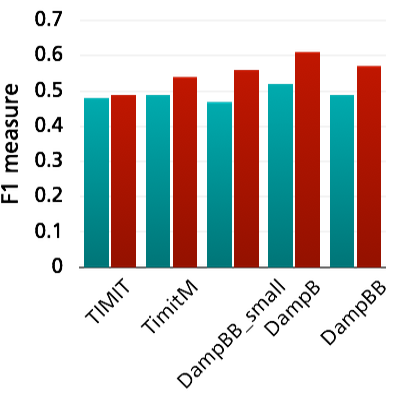
\includegraphics[width=\textwidth]{images/kws_exp4_acap.png}
                \caption{$F_1$ measures for keyword spotting results on the \textit{ACAP} data set with post-processor duration modeling.}
                \label{fig:kws_exp4_acap}
                
        \end{subfigure}%
         %add desired spacing between images, e. g. ~, \quad, \qquad, \hfill etc.
          %(or a blank line to force the subfigure onto a new line)
        \begin{subfigure}[t]{0.5\textwidth}
                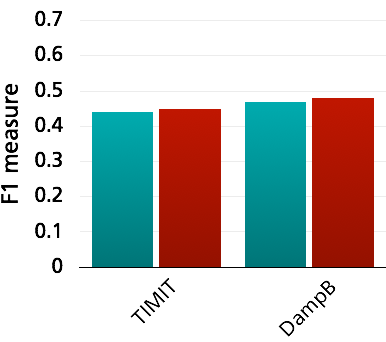
\includegraphics[width=\textwidth]{images/kws_exp4.png}
                \caption{$F_1$ measures for keyword spotting results on the \textit{DampTest} data sets with post-processor duration modeling.}
                \label{fig:kws_exp4}
                
        \end{subfigure}
        \caption{$F_1$ measures for keyword spotting results using posteriorgrams generated with various acoustic models with post-processor duration modeling.}
          \end{figure}


Results with and without post-processor duration modeling for the \textit{ACAP} data set are shown in figure \ref{fig:kws_exp4_acap}. All models were tested. As these results show, $F_1$ measures improve for all configurations when post-processor duration modeling is employed. The effect is somewhat stronger for the \textit{DAMP} models than for the \textit{TIMIT} model. This confirms that those models are, in principle, able to detect the keyword phonemes, and that exploiting information about plausible phoneme durations can improve the precision. The best result rises from $0.52$ to $0.61$ with the \textit{DampB} model. Analysis of the detailed results shows that the precision can be improved significantly when detected occurrences with implausible phoneme durations are discarded. However, this often also decreases the recall, resulting in the shown $F_1$ results.\\

The approach was also tested on the \textit{DampTest} data sets for two acoustic models. As seen above, $F_1$ measures on these data sets are generally somewhat blurry for the described reasons. In this case, the results are just a little bit higher with post-processor duration modeling.


%TODO: clean up
\section{Conclusion}\label{sec:kws_conclusion}
%insgesamt besser
%huge DampB set best, but 3% DampBB almost as good
% even v small DampBB_small better than Timit
% context does not help
% gender models slightly better for kws, not better for phone rec --> variability?
% results phonerec
% results kws - esp. interesting because short
%---auto alignment error source


In this chapter, an approach for keyword spotting using the new acoustic models trained on singing was described. This was done by extracting phoneme posteriorgrams generated with these new models from the audio and then running them through a keyword-filler approach to detect 15 keywords. The resulting $F_1$ measure rises from $0.44$ for the models trained on speech (\textit{TIMIT}) to $0.47$ for the new models. This result is especially interesting because most of the keywords have few phonemes. Gender-dependent models perform very slightly better than mixed-gender models of the same size. Individual analysis of the keyword results showed that keywords that occur more frequently are detected more accurately. This probably happens because the approach is able to obtain high recall easily, but precision is an issue. The more frequent a keyword, the easier obtaining higher precisions becomes. Additionally, keywords with more phonemes are detected more accurately than short ones because there is more information to base detection on.\\

The approach was further expanded by including duration information. 

This approach was only tested with MFCC features. As preliminary experiments suggest \cite{kruspe_kws1}, other features like TRAP or PLP may work better on singing. So-called log-mel filterbank features have also been used successfully with DNNs \cite{hinton}. Another interesting factor is the size and configuration of the classifiers, of which only one was tested (after a small grid search to validate this choice). Other experiments also suggest that incorporating certain phoneme duration information into the recognition can improve the over-all results \cite{kruspe_kws2}.\\
As in the phoneme recognition experiments, there is only a slight amount of improvement between the acoustic model trained on all 6000 songs of the \textit{DAMP} data set and the one trained only on $4\%$ of this data. It would be interesting to find the exact point at which additional training data does not further improve the models. On the evaluation side, a keyword spotting approach that allows for pronunciation variants or sub-words may produce better results. Language modeling might also help to alleviate some of the errors made during phoneme recognition.\\
These models have not yet been applied to singing with background music, which would be interesting for practical applications. Since this would probably decrease the result when used on big, unlimited data sets, more specified systems would be more manageable, e.g. for specific music styles, sets of songs, keywords, or specialized applications. Searching for whole phrases instead of short keywords could also make the results better usable in practice.\\
As shown in \cite{mesaros_alignment} and \cite{goto_alignment} and in the next chapter, alignment of textual lyrics and singing already works well. A combined approach that also employs textual information could be very practical.

